%%%%%%%%%%%%%%%%%%%% author.tex %%%%%%%%%%%%%%%%%%%%%%%%%%%%%%%%%%%
%
% sample root file for your "contribution" to a contributed volume
%
% Use this file as a template for your own input.
%
%%%%%%%%%%%%%%%% Springer %%%%%%%%%%%%%%%%%%%%%%%%%%%%%%%%%%


% RECOMMENDED %%%%%%%%%%%%%%%%%%%%%%%%%%%%%%%%%%%%%%%%%%%%%%%%%%%
\documentclass[graybox]{svmult}

% choose options for [] as required from the list
% in the Reference Guide

\usepackage{type1cm}        % activate if the above 3 fonts are
                            % not available on your system
%
\usepackage{makeidx}         % allows index generation
\usepackage{graphicx}        % standard LaTeX graphics tool
                             % when including figure files
\usepackage{multicol}        % used for the two-column index
\usepackage[bottom]{footmisc}% places footnotes at page bottom


\usepackage{newtxtext}       % 
\usepackage{newtxmath}       % selects Times Roman as basic font

\usepackage{booktabs}       % Booktabs Table Style
	
\usepackage{graphicx}       % To frame graphic images
\usepackage[export]{adjustbox}

\usepackage[section]{placeins} % Forces an image to be displayed in it's section


% see the list of further useful packages
% in the Reference Guide

\makeindex             % used for the subject index
                       % please use the style svind.ist with
                       % your makeindex program

%%%%%%%%%%%%%%%%%%%%%%%%%%%%%%%%%%%%%%%%%%%%%%%%%%%%%%%%%%%%%%%%%%%%%%%%%%%%%%%%%%%%%%%%%

\DeclareUnicodeCharacter{2212}{-}
\DeclareUnicodeCharacter{22C5}{-}

\begin{document}
\title{Recovering from population extinction in the Animal Life Cycle Algorithm (ALCA)}
%


\titlerunning{Animal Life Cycle Algorithm (ALCA)}
% Use \titlerunning{Short Title} for an abbreviated version of
% your contribution title if the original one is too long
\author{J. C. Felix-Saul, Mario Garcia Valdez}
% Use \authorrunning{Short Title} for an abbreviated version of
% your contribution title if the original one is too long
\institute{J. C. Felix-Saul \at Tijuana Institute of Technology, Tijuana, Mexico, \email{jose.felix201@tectijuana.edu.mx}
\and Mario García Valdez \at Tijuana Institute of Technology, Tijuana, Mexico, \email{mario@tectijuana.edu.mx}}
%
% Use the package "url.sty" to avoid
% problems with special characters
% used in your e-mail or web address
%
\maketitle

\abstract*{In previous work, we introduced an algorithm inspired by the
biological Life Cycle of animal species, consisting of the stages: birth,
growth, reproduction, and death. As in nature, population individuals grow
older and age. In this algorithm's reproduction process, couples must match by
mutual attraction, where sometimes individuals won't procreate offspring
because of the mate's low appeal. As time passes, the environment kills its
individuals either because of low fitness or age, causing occasional population
extinction. When this condition presents, it is required to create a new
population if evaluations are available and termination conditions are
favorable to continue. Some alternatives we explored to restart this new
population are the random generation of a new set of candidate solutions and
the creation of a new set of candidate solutions based on either: a mix of
elements from the best historically found candidate solutions set (Elite); the
mutation with uniform modification from the Elite or the historically
best-found solution (Champion); crossing the Champion with the Elite; the
projection of the Elite towards the Champion; based on random use of the
previous alternatives. In this paper, we present one of the most promising
alternatives to solve population extinction caused by nature's pressure in the
Life Cycle algorithm: the projection of the Elite towards the Champion, where
we compare the results obtained with the latter and the random use of all the
alternatives, using classic benchmark functions for optimization for
comparison.}



\abstract{In previous work, we introduced an algorithm inspired by the
biological Life Cycle of animal species, consisting of the stages: birth,
growth, reproduction, and death. As in nature, population individuals grow
older and age. In this algorithm's reproduction process, couples must match by
mutual attraction, where sometimes individuals won't procreate offspring
because of the mate's low appeal. As time passes, the environment kills its
individuals either because of low fitness or age, causing occasional population
extinction. When this condition presents, it is required to create a new
population if evaluations are available and termination conditions are
favorable to continue. Some alternatives we explored to restart this new
population are the random generation of a new set of candidate solutions and
the creation of a new set of candidate solutions based on either: a mix of
elements from the best historically found candidate solutions set (Elite); the
mutation with uniform modification from the Elite or the historically
best-found solution (Champion); crossing the Champion with the Elite; the
projection of the Elite towards the Champion; based on random use of the
previous alternatives. In this paper, we present one of the most promising
alternatives to solve population extinction caused by nature's pressure in the
Life Cycle algorithm: the projection of the Elite towards the Champion, where
we compare the results obtained with the latter and the random use of all the
alternatives, using classic benchmark functions for optimization for
comparison.}

%\keywords{Distributed Bioinspired Algorithms \and Genetic Algorithms \and Cloud Computing.}

\newpage
\section{Introduction}
    \label{sec:1}

    Biologically inspired algorithms have proven to be very effective when
    solving complex optimization problems
    \cite{castillo2019comparative,valdez2021swarm,acherjee2020ultrasonic}, but
    the more challenging the problem, the more computing power it will require
    to solve them \cite{ontiveros2018high}. We consider the main reason it requires 
    more computing power is related to the evaluation of the fitness function, 
    which means calculating the solution to the real problem our algorithm is searching for. 
    One technique to manage this
    processing power demand is to use distributed computing
    \cite{thain2005distributed} or the cloud resources 
    \cite{garcia2013there,eshratifar2019bottlenet}. This strategy allows adaptation 
    of the required computing need according to the problem's complexity.
    
    Traditionally, bio-inspired algorithms are developed with a sequential
    (synchronous) perspective
    \cite{porto2018evolutionary,back1996evolutionary}, where a process must
    pause for the previous task to finish before continuing. 
    Some architectures address this issue \cite{valdez2021container,garcia2015evospace,merelo2016nodio} 
    by working on the cloud and finding solutions on distributed technologies.
    In this research, we present a distributed algorithm totally built as a 
    native cloud solution, where its processes execute asynchronously and in 
    parallel, managing the processing workload among several computers.  
    This strategy allows to elastically increase (or reduce) the
    computing power according to the nature of the challenge
    \cite{armbrust2010view}.

    In previous work, we introduced an algorithm inspired by the biological
    life-cycle of animal species \cite{Felix-Saul2022}. As in nature, population individuals grow older
    and age. In this algorithm's reproduction process, couples must match by mutual
    attraction, where sometimes individuals won't procreate offspring because of
    the mate's low appeal. As time passes, the environment kills its individuals
    either because of low fitness or age, causing occasional population extinction.
    % Just to be sure explain a bit more what we mean by extinsion. - M
    When this condition presents itself, it is required to create a new population
    to continue evolution (restart). 
    % Maybe you do it later, but explain what is a restart precisely 
    In a previous work \cite{Felix-Saul2022} we used to generate a new random
    set of solutions, with the cost of losing all evolution knowledge.

    One contribution of this paper is to demonstrate that it is possible to
    evolve a population of individuals, similar to a Genetic Algorithm (GA),
    using a distributed, parallel, and asynchronous methodology by algorithm
    implementation and testing.

    The main contribution of this research is to demonstrate how to improve the
    algorithm's behavior, by solving population extinction caused by nature's
    pressure in the Animal Life Cycle Algorithm with one of the most promising
    alternatives: the projection of the Elite towards the Champion. To validate
    our findings, we compare the results obtained with the latter and the
    random use of the more traditional alternatives (mutation and crossover),
    using classic benchmark functions for optimization for comparison.

    This paper is organized as follows. First, we 
    illustrate our algorithm model, the encountered problem with the occasional
    population extinction, and our proposed solution in
    section~\ref{section.proposal}, followed by our experimental configuration and
    results in section~\ref{section.experiments}, where we continue to analyze and
    describe some of our research findings in section~\ref{section.discussion}. We
    finalize by presenting some inferences based on the results of our experiments
    in section~\ref{section.conclusions}.

    % If we are not going to add a State of the Art section, we need to mention other 
    % methods in the Introduction. - M
\section{Proposal}
    \label{section.proposal}

    In previous work, we presented an algorithm inspired by nature 
    \cite{Felix-Saul2022}, where we model our algorithm based on
    the generalization of the life cycle of animal species. Our algorithm, as
    in nature, consists of four stages \cite{read1968system}: birth, growth,
    reproduction, and death. One key concept of our idea is that combining
    those processes evolves the population. We propose to execute all these
    stages in parallel and asynchronously on a continuously evolving
    population.


    \subsection{Algorithm Model}
        
        This algorithm was inspired by the traditional Genetic Algorithm,
        meaning that all individuals have a genotype (chromosome) that is a
        list of values. We calculate the individual's fitness with the
        evaluation function and do crossover and mutation to the population.
        What makes our strategy different is that we don't use the concept of
        evolutionary generations. We manage our set of solutions as a whole
        that continuously evolve over time. Allowing individuals of different
        ages to breed and generate offspring, as it happens in nature. The
        crossover and mutation execute as independent processes that randomly
        affect the individuals.

        Our algorithm's goal is to mimic the animal life cycle, where at any
        given moment, new individuals are born to be part of the population and
        participate in the collective evolution. As time passes, they grow
        older and mature, suffering changes throughout their lives that we
        chose to represent as mutations. In our analysis, we considered a
        couple's attraction a fundamental factor in reproduction. We thought of
        death's work to maintain balance in the population by enforcing the
        survival of the fittest. As in life, death can happen to everyone: from
        a newborn to the elderly, where fitness will determine the individual's
        longevity. We display the general model concept in
        Figure~\ref{fig.algorithm_model}.
        % I do not like that image, is not very clear. We are confused by the 
        % similarity with Venn diagrams. Maybe is better to put boxes and arrows. - M

        \subsubsection{Birth} Birth is the first step of the population's
        evolution. For the algorithm representation, we begin with the
        generation of a randomly set of individuals.
        
        \subsubsection{Growth} In our algorithm representation, there is a
        direct correlation between elapsed time and the population's evolution.
        For this to be possible in our proposal, all individuals must grow
        older and change as time progresses. With each increment of age, an
        individual may improve or deteriorate. We chose to manifest this idea
        by performing a small mutation in each change.

        \subsubsection{Reproduction} In this step, we select a random pair of
        individuals and evaluate their couple's attraction, where fitness will
        be the decisive factor that impacts its value. The higher the fitness
        of the individual, the more attractive it will appear to fellow
        individuals. As a consequence of the previous concept, we can
        anticipate that not all couples will produce offspring, meaning
        reproduction will not always be successful.
        
        \subsubsection{Death} Death is the last step of the animal life cycle,
        as in our algorithm. We chose death as a representation of all the
        environmental challenges for survival, where its execution enforces the
        survival of the fittest. As time progresses, so does increase nature's
        level of danger. The better the individual fitness will increase its
        chances of survival.
        
        \begin{figure}
            \centering
            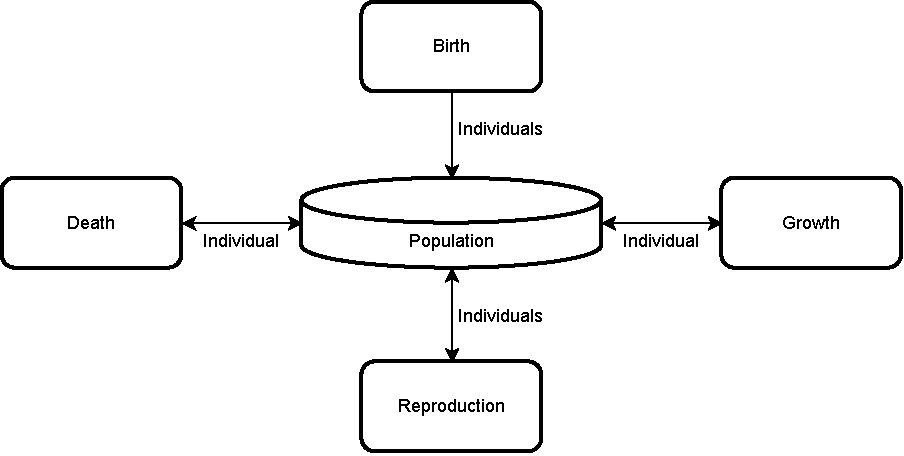
\includegraphics[width=80mm]{img/fig_algorithm_model.pdf}
            \caption{Animal Life Cycle Algorithm model.} \label{fig.algorithm_model}
            \end{figure}

    \subsection{Problem}

        In this algorithm's reproduction process, we find mating couples by mutual
        attraction, where sometimes individuals won't procreate offspring because of
        the mate's low appeal. As time passes, the environment could kill its
        individuals either because they have low fitness or age, leading to extinction,
        meaning there are no more individuals in the population left to reproduce. When
        this condition presents, if evaluations are available and termination
        conditions enable the algorithm to continue the search, it is required to
        create a new set of individuals. We illustrate the general flowchart for the
        Life-Cycle algorithm in Figure~\ref{fig.flowchart}.
        

        \begin{figure}
            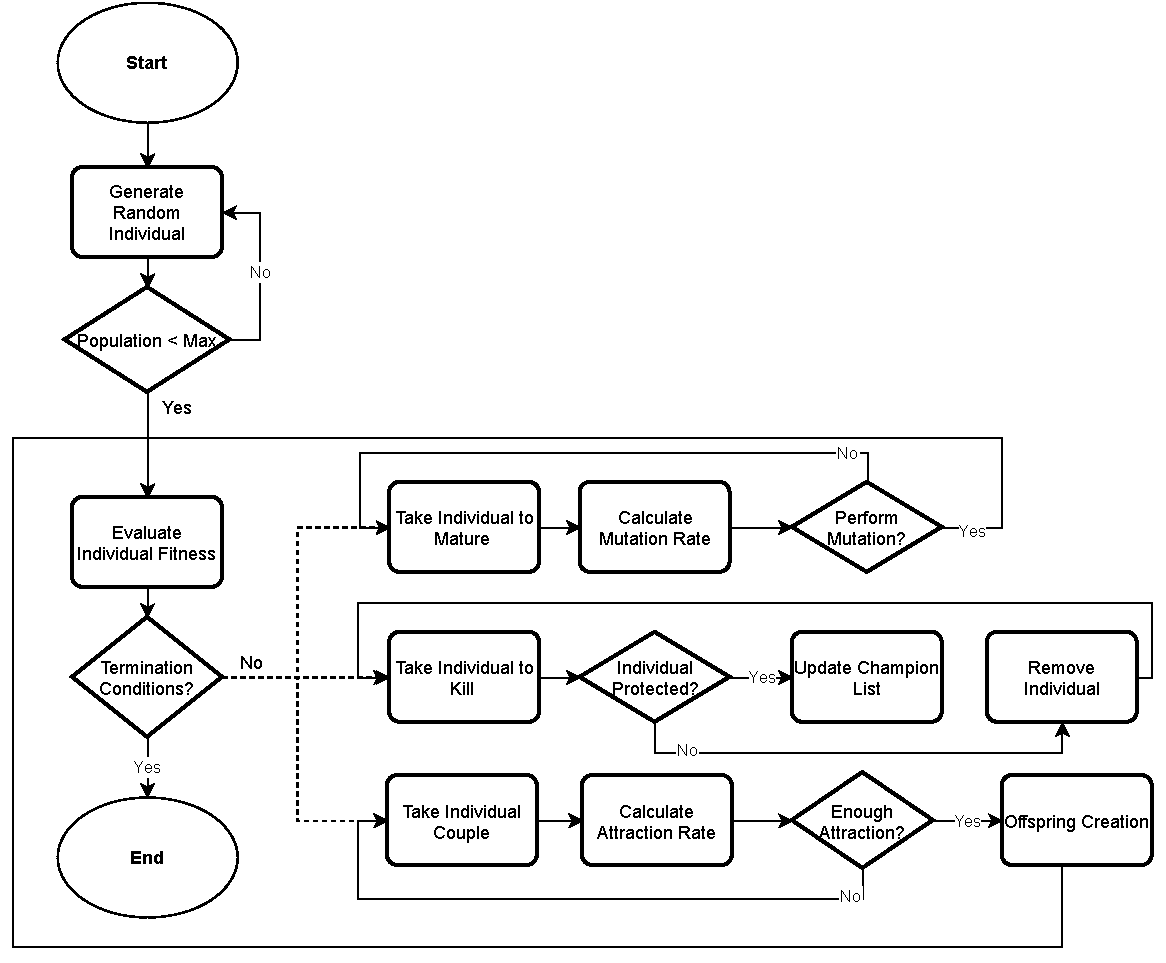
\includegraphics[width=\textwidth]{img/fig_flowchart.pdf}
            \caption{Animal Life-Cycle Algorithm general flowchart.} \label{fig.flowchart}
            \end{figure}

    \subsection{Proposed Solution}
        % It is important to do a literature review for the following papers, there are 
        % other works that tackle similar problems or use it as a strategy. - M 
        In this article, we test various strategies to generate a new population to
        replace individuals that have already died (or were discarded) due to their
        aptitude, as happens in the life cycle. We previously used to generate a new
        random set of solutions, with the cost of losing all evolution knowledge. 
        
        This article proposes some strategies to carry out this operation,
        where the presented distribution strategy obtained the best results. We
        propose one promising alternative to restart the population, to solve
        extinction caused by nature's pressure in the Life Cycle algorithm: the
        projection of the historically best-found candidate solutions (Elite)
        towards the best-found candidate solution (Champion).

        The strategy we describe in this paper use an elite set, that includes
        the historically best-found candidate solutions to take
        advantage of the historical evolution. Our goal is for the offspring to
        be somewhat close to the best individuals of the Elite.
        We use the golden ratio to compute the distance between new individuals in the population, making
        an improved distribution. We can consider our strategy an improvement 
        over other alternatives because of the findings of our latter experiments.

        Based on the historically best candidate
        solution and the elite set, we use the Golden Ratio (shown in
        Figure~\ref{fig.golden_ratio}) to compute the distance between new individuals
        in the population, making an improved distribution. It randomly selects a
        solution from the elite set and uses the Golden Ratio 
        \cite{nematollahi2020novel, gaikwad2021face, khesin2022golden, sym13081334, https://doi.org/10.1111/nyas.14895} 
        to compute multiple solutions against the best-found candidate.

        \begin{figure}
            \centering
            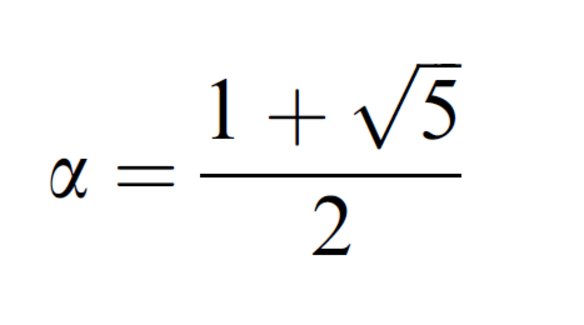
\includegraphics[width=25mm]{img/fig_golden_ratio.pdf}
            \caption{Golden Ratio equation.} \label{fig.golden_ratio}
            \end{figure}

        This strategy is how we can calculate the projection of the
        historically Elite towards the Champion solution. To illustrate this
        concept, we include Figure~\ref{fig.elite_projection}, placing the
        Elite solution on the far right and the Champion solution on the left
        corner. We can observe the higher amount of new solutions progressively
        closer to the Champion.
        
        \begin{figure}
            \centering
            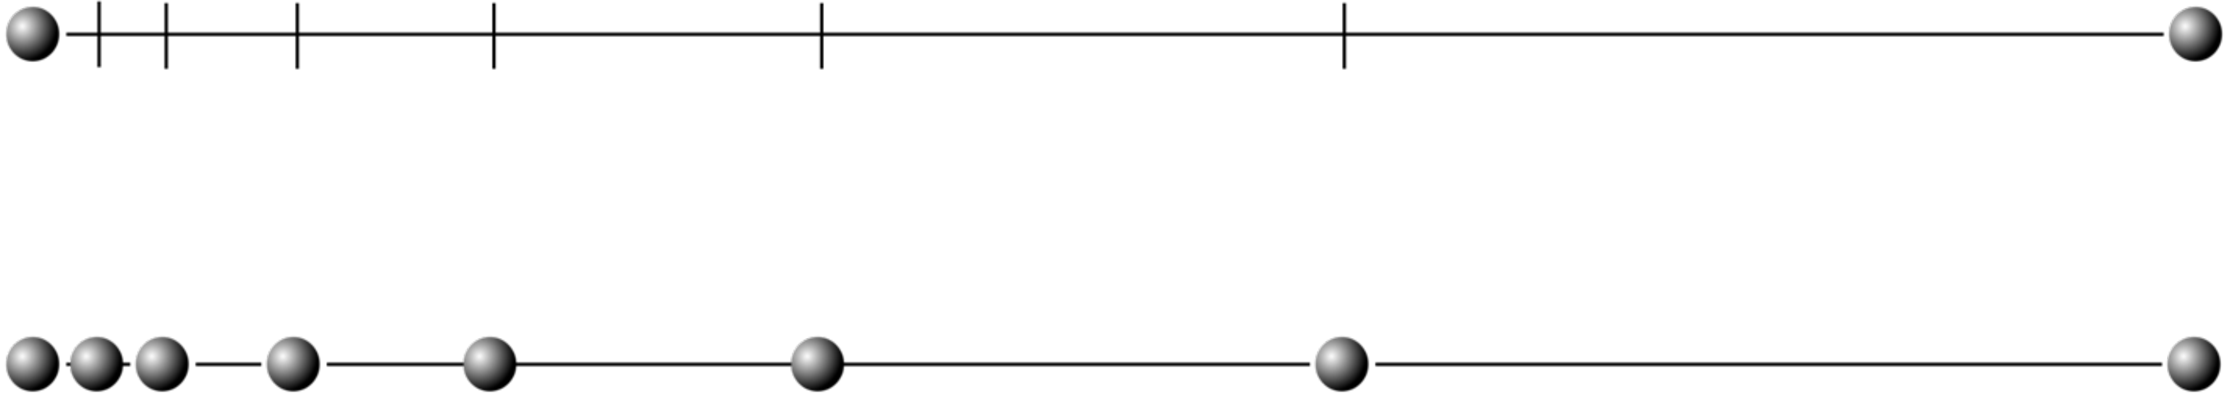
\includegraphics[width=0.65\textwidth]{img/fig_elite_projection.pdf}
            \caption{Projection of an Elite solution (found on the right) towards the Champion (at the left).} \label{fig.elite_projection}
            \end{figure}

        This process generates new solutions that will be the new population set. It
        uses the Golden Ratio to progressively approximate from an Elite solution to
        the Champion. This strategy facilitates to find apparently hidden solutions,
        having an exploitation emphasis. Figure~\ref{fig.elite_projection_swarm}
        displays the projection of five Elite solutions (on the corners) towards the
        Champion (in the center).

        \begin{figure}
            \centering
            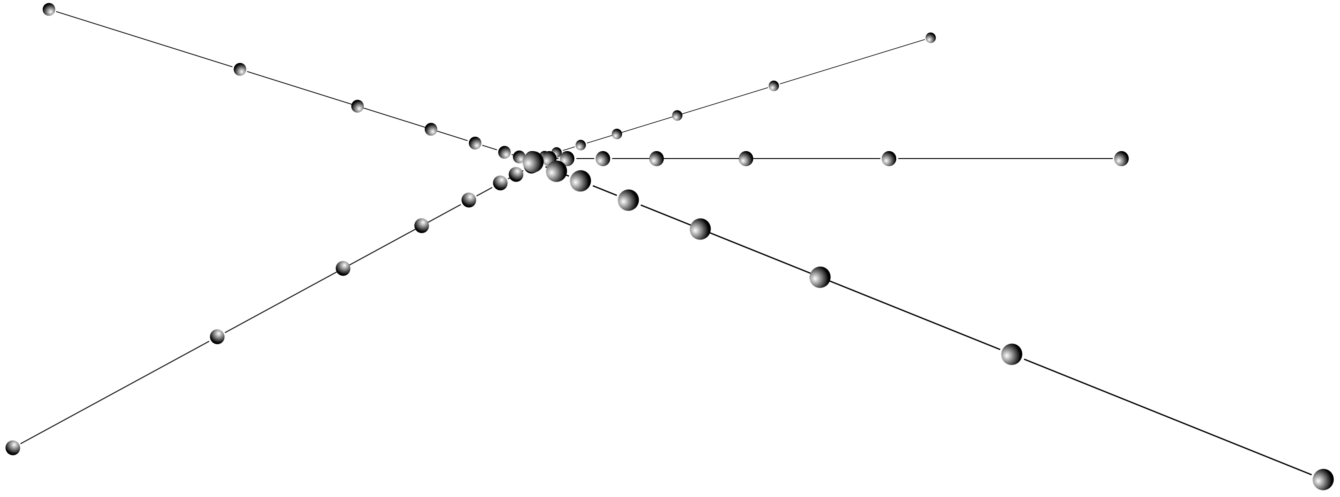
\includegraphics[width=0.85\textwidth]{img/fig_elite_projection_swarm.pdf}
            \caption{Projection of five Elite solutions towards the Champion, results in a mini-swarm.} \label{fig.elite_projection_swarm}
            \end{figure}
        
        \FloatBarrier

\section{Experiments}
    \label{section.experiments}

    As a proof-of-concept, we implemented the algorithm with Docker containers,
    where we compare the results obtained with the projection of the Elite towards
    the Champion strategy and the random use of the more traditional alternatives
    (such as mutation and crossover), using classic benchmark functions for
    optimization as implemented by the DEAP (Distributed Evolutionary Algorithms in
    Python) library \cite{fortin2012deap}.

    \subsection{Experimental Setup} 

        The following tables show the configuration used to execute the experiments for
        the analysis and comparison in this paper. In
        Table~\ref{tab.general_configuration}, we can find the General Configuration
        for the Animal Life Cycle Algorithm. All values from this configuration
        remained constant during all phases of the experiment runs. The following
        table, Table~\ref{tab.benchmark_fun_config}, shows the values used for the
        Classic Benchmark Functions for Optimization, where these are adjusted
        accordingly for each function.

        % Please add the following required packages to your document preamble:
        % \usepackage{booktabs}
        % To change the size of the font use \scriptsize or \tiny
        \begin{table}[]
            \scriptsize
            \centering
            \caption{Animal Life Cycle Algorithm (ALCA) General Configuration.}\label{tab.general_configuration}
            \begin{tabular}{@{}ll@{}}
            \toprule
            \multicolumn{2}{l}{\textbf{ALCA General Configuration}} \\ \midrule
            Function name & ALL \\
            Population & 500 \\
            Target error & 1.00E-08 \\
            Crossover rate & 100 \\
            Mutation rate & 7 \\
            Max age & 40 \\
            Tournament rep. & 100 \\
            Sample size & 20 \\
            Base approval & 80 \\
            Goal approval & 200 \\ \bottomrule
            \end{tabular}
            \end{table}

        \begin{table}[]
            \scriptsize
            \centering
            \caption{Classic Benchmark Functions for Optimization Configuration.}\label{tab.benchmark_fun_config}
            \begin{tabular}{@{}llllllll@{}}
            \toprule
            \multicolumn{8}{l}{\textbf{Benchmark Configuration Setup}} \\ \midrule
            Function name & Ackley & Bohachevsky & Griewank & Rastrigin & Sphere & Rosenbrock & Rosenbrock \\
            Dimensions & 5, 10 & 5, 10 & 5, 10 & 5, 10 & 5, 10 & 5 & 10 \\
            Max evaluations & 200,000 & 200,000 & 200,000 & 200,000 & 200,000 & 500,000 & 1,000,000 \\
            Max stagnation & 50,000 & 50,000 & 50,000 & 50,000 & 50,000 & 125,000 & 250,000 \\
            Target fitness & -20.0 & -12.0 & -150.0 & -80.0 & -50.0 & -3500.0 & -3500.0 \\
            Bound matrix & {[}-32, 32{]} & {[}-2, 2{]} & {[}-500, 500{]} & {[}-5, 5{]} & {[}-5, 5{]} & {[}-2, 2{]} & {[}-2, 2{]} \\ \bottomrule
            \end{tabular}
            \end{table}
        
        \FloatBarrier


    \subsection{Experiment Results}

        For each experiment, we ran 30 independent executions per algorithm and
        dimensions specified. We recorded the following results: best found error,
        standard deviation, total number of evaluations, and total elapsed time (in
        seconds). The labels used on the results of our summarized experiments tables
        are the following:

        \begin{itemize}
            \item   Error:       is the best found error (or best solution).
            \item   St-Dev:      is the standard deviation calculated from the error. 
            \item   Evals.:      is the total number of evaluations the algorithm executed.
            \item   Time:        is the total elapsed or wall clock time, in seconds. 
        \end{itemize}

        The alternatives to restart this new population are the creation of a new set
        of candidate solutions based on either: 1. Crossing the Champion with the Elite;
        2. The mutation with uniform modification from the Elite; 3. The
        projection of the Elite towards the Champion; 4. Based on random use of the
        previous alternatives. We compared three strategies by grouping the previous
        alternatives in the following:

        \begin{itemize}
            \item   Xover Mutation:      Crossing the Champion with the Elite, and the mutation with uniform modification from the Elite.
            \item   Elite Projection:    The projection of the Elite towards the Champion. 
            \item   All Random:          Based on random use of the previous alternatives.
        \end{itemize}

        \subsubsection{Ackley Benchmark Function Experiment}

            The goal of the first experiment was to confirm that this paper’s
            proposed strategy obtained improved results over our basic
            technique, which created a new population with a random generation
            of a new set of candidate solutions. We chose Ackley as the first
            Classic Benchmark Function for Optimization to test our algorithm
            behavior, where Figure~\ref{fig.fun_ackley} shows its corresponding
            Box and Whisker chart, and we summarized the results in
            Tables~\ref{tab.fun_ackley5} and~\ref{tab.fun_ackley10} (for five 
            and ten dimensions, respectively).
            
            \begin{figure}
                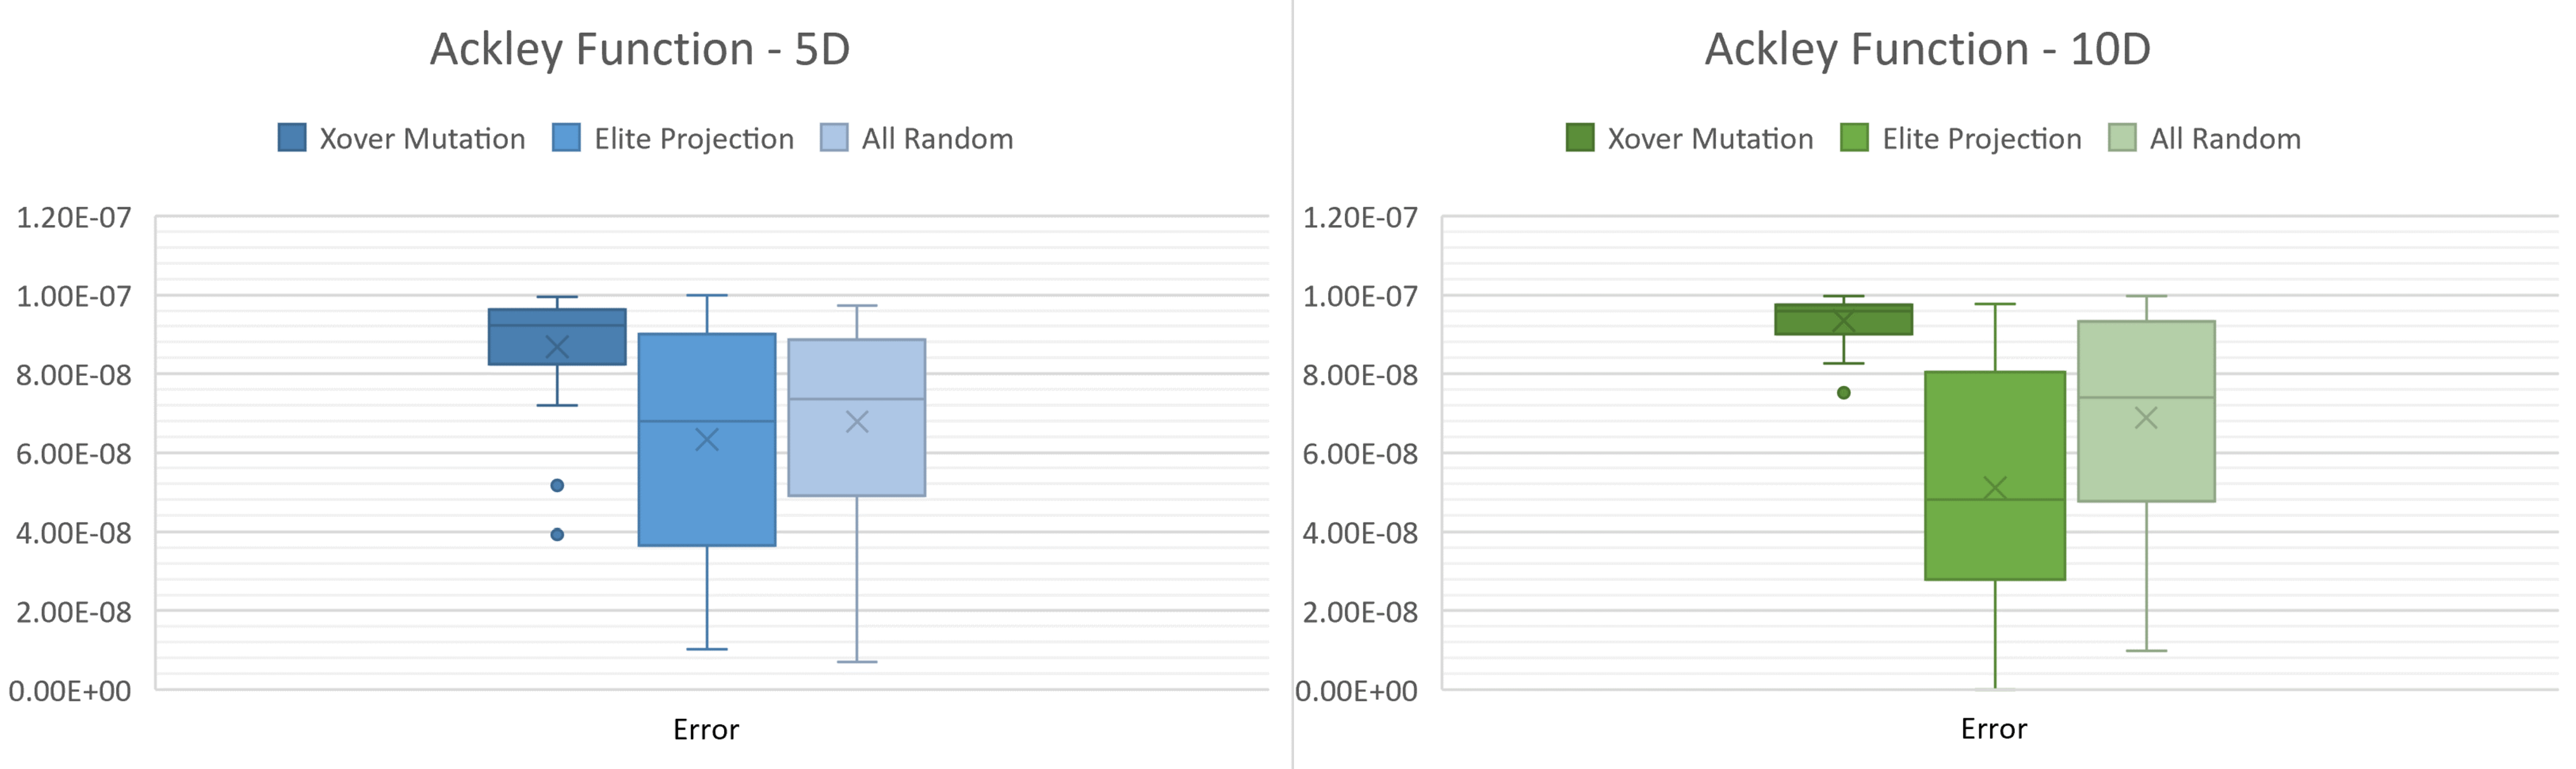
\includegraphics[width=0.99\linewidth, frame]{img/fig_fun_ackley.pdf}
                \caption{Box and whisker chart for the Ackley Benchmark Function, 5 vs 10 Dimensions.} \label{fig.fun_ackley}
                \end{figure}

            \begin{table}[]
                \scriptsize
                \centering
                \caption{Ackley Benchmark Function summarized experiments table for 5 Dimensions.}\label{tab.fun_ackley5}
                \begin{tabular}{@{}lllll@{}}
                \toprule
                \multicolumn{5}{l}{\textbf{Ackley Function - 5 Dimensions}} \\ \midrule
                & \textbf{Error} & \textbf{St-Dev} & \textbf{Evals.} & \textbf{Time} \\
                \textbf{Xover Mutation} & 8.69E-08 & 1.36E-08 & 46,331 & 49.9 \\
                \textbf{Elite Projection} & 6.33E-08 & 2.70E-08 & 13,811 & 18.1 \\
                \textbf{All Random} & 6.78E-08 & 2.55E-08 & 30,236 & 32.8 \\ \bottomrule
                \end{tabular}
                \end{table}

            \begin{table}[]
                \scriptsize
                \centering
                \caption{Ackley Benchmark Function summarized experiments table for 10 Dimensions.}\label{tab.fun_ackley10}
                \begin{tabular}{@{}lllll@{}}
                \toprule
                \multicolumn{5}{l}{\textbf{Ackley Function - 10 Dimensions}} \\ \midrule
                & \textbf{Error} & \textbf{St-Dev} & \textbf{Evals.} & \textbf{Time} \\
                \textbf{Xover Mutation} & 9.35E-08 & 5.93E-09 & 104,842 & 111.7 \\
                \textbf{Elite Projection} & 5.11E-08 & 3.13E-08 & 16,019 & 20.1 \\
                \textbf{All Random} & 6.89E-08 & 2.75E-08 & 43,631 & 46.3 \\ \bottomrule
                \end{tabular}
                \end{table}
            
            \FloatBarrier


        \subsubsection{Bohachevsky Benchmark Function Experiment}

            As our second experiment to further validate and prove our
            algorithm behavior, we chose Bohachevsky Classic Benchmark Function
            for Optimization. Figure~\ref{fig.fun_bohachevsky} shows its
            corresponding Box and Whisker chart, where we summarized the
            results in Tables~\ref{tab.fun_bohachevsky5} and~\ref{tab.fun_bohachevsky10} 
            (for five and ten dimensions, respectively). Due to the observation 
            and analysis of these results, we identify our proposed strategy 
            obtained solutions in the same order as the traditional Xover Mutation, 
            in a significantly reduced number of evaluations.

            \begin{figure}
                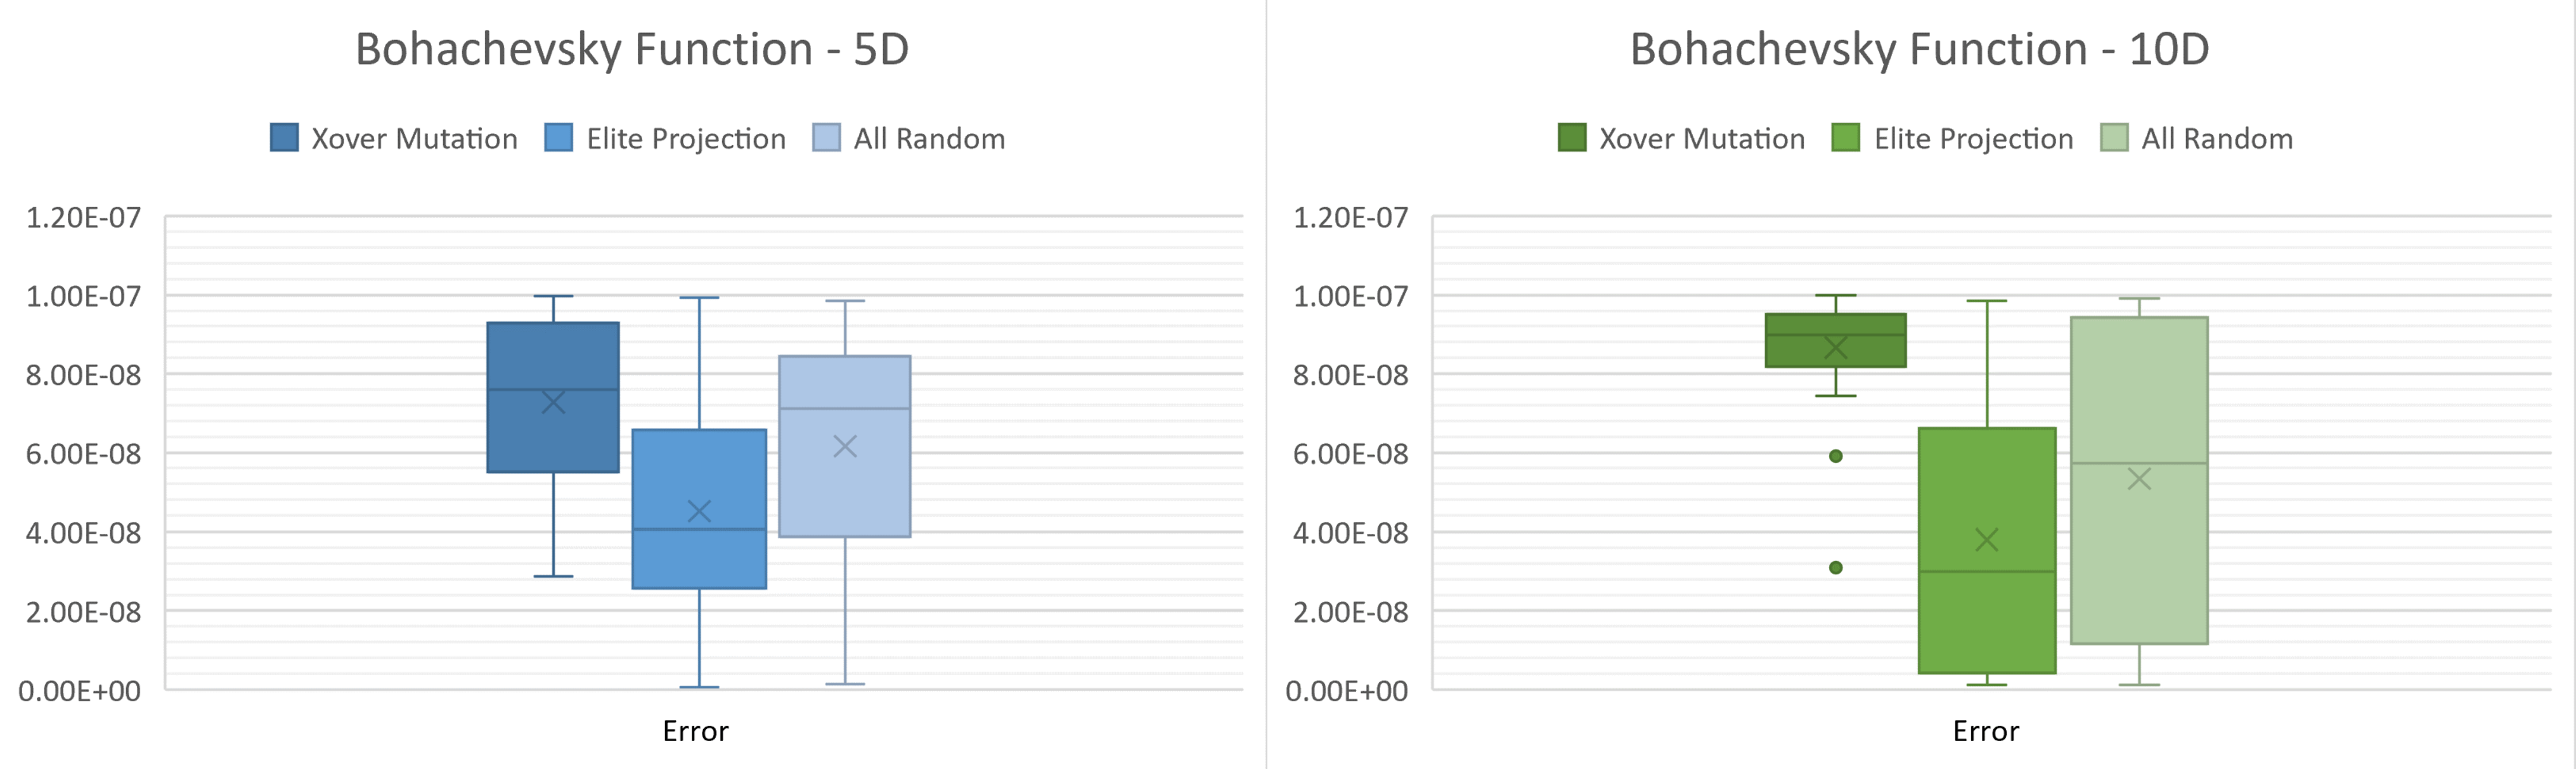
\includegraphics[width=0.99\linewidth, frame]{img/fig_fun_bohachevsky.pdf}
                \caption{Box and whisker chart for the Bohachevsky Benchmark Function, 5 vs 10 Dimensions.} \label{fig.fun_bohachevsky}
                \end{figure}

            \begin{table}[]
                \scriptsize
                \centering
                \caption{Bohachevsky Benchmark Function summarized experiments table for 5 Dimensions.}\label{tab.fun_bohachevsky5}
                \begin{tabular}{@{}lllll@{}}
                \toprule
                \multicolumn{5}{l}{\textbf{Bohachevsky Function - 5 Dimensions}} \\ \midrule
                & \textbf{Error} & \textbf{St-Dev} & \textbf{Evals.} & \textbf{Time} \\
                \textbf{Xover Mutation} & 7.28E-08 & 2.20E-08 & 15,010 & 24.2 \\
                \textbf{Elite Projection} & 4.51E-08 & 2.94E-08 & 8,266 & 12.6 \\
                \textbf{All Random} & 6.16E-08 & 2.85E-08 & 11,998 & 21.7 \\ \bottomrule
                \end{tabular}
                \end{table}

            \begin{table}[]
                \scriptsize
                \centering
                \caption{Bohachevsky Benchmark Function summarized experiments table for 10 Dimensions.}\label{tab.fun_bohachevsky10}
                \begin{tabular}{@{}lllll@{}}
                \toprule
                \multicolumn{5}{l}{\textbf{Bohachevsky Function - 10 Dimensions}} \\ \midrule
                & \textbf{Error} & \textbf{St-Dev} & \textbf{Evals.} & \textbf{Time} \\
                \textbf{Xover Mutation} & 8.66E-08 & 1.38E-08 & 40,166 & 44.4 \\
                \textbf{Elite Projection} & 3.80E-08 & 3.34E-08 & 8,506 & 12.9 \\
                \textbf{All Random} & 5.34E-08 & 3.76E-08 & 19,537 & 26.8 \\ \bottomrule
                \end{tabular}
                \end{table}
            
            \FloatBarrier


        \subsubsection{Griewank Benchmark Function Experiment}

            The third experiment objective was to confirm Animal Life Cycle
            Algorithm continued finding solutions in a reduced number of
            evaluations. For this test, we selected the Griewank Benchmark
            Function for Optimization. Figure~\ref{fig.fun_griewank} shows its
            corresponding Box and Whisker chart, where we summarized the
            results in Tables~\ref{tab.fun_griewank5} and~\ref{tab.fun_griewank10} 
            (for five and ten dimensions, respectively). With this analysis, 
            we confirmed our strategy continued to obtain solutions in the same 
            order as expected, in a reduced number of evaluations and less time.

            \begin{figure}
                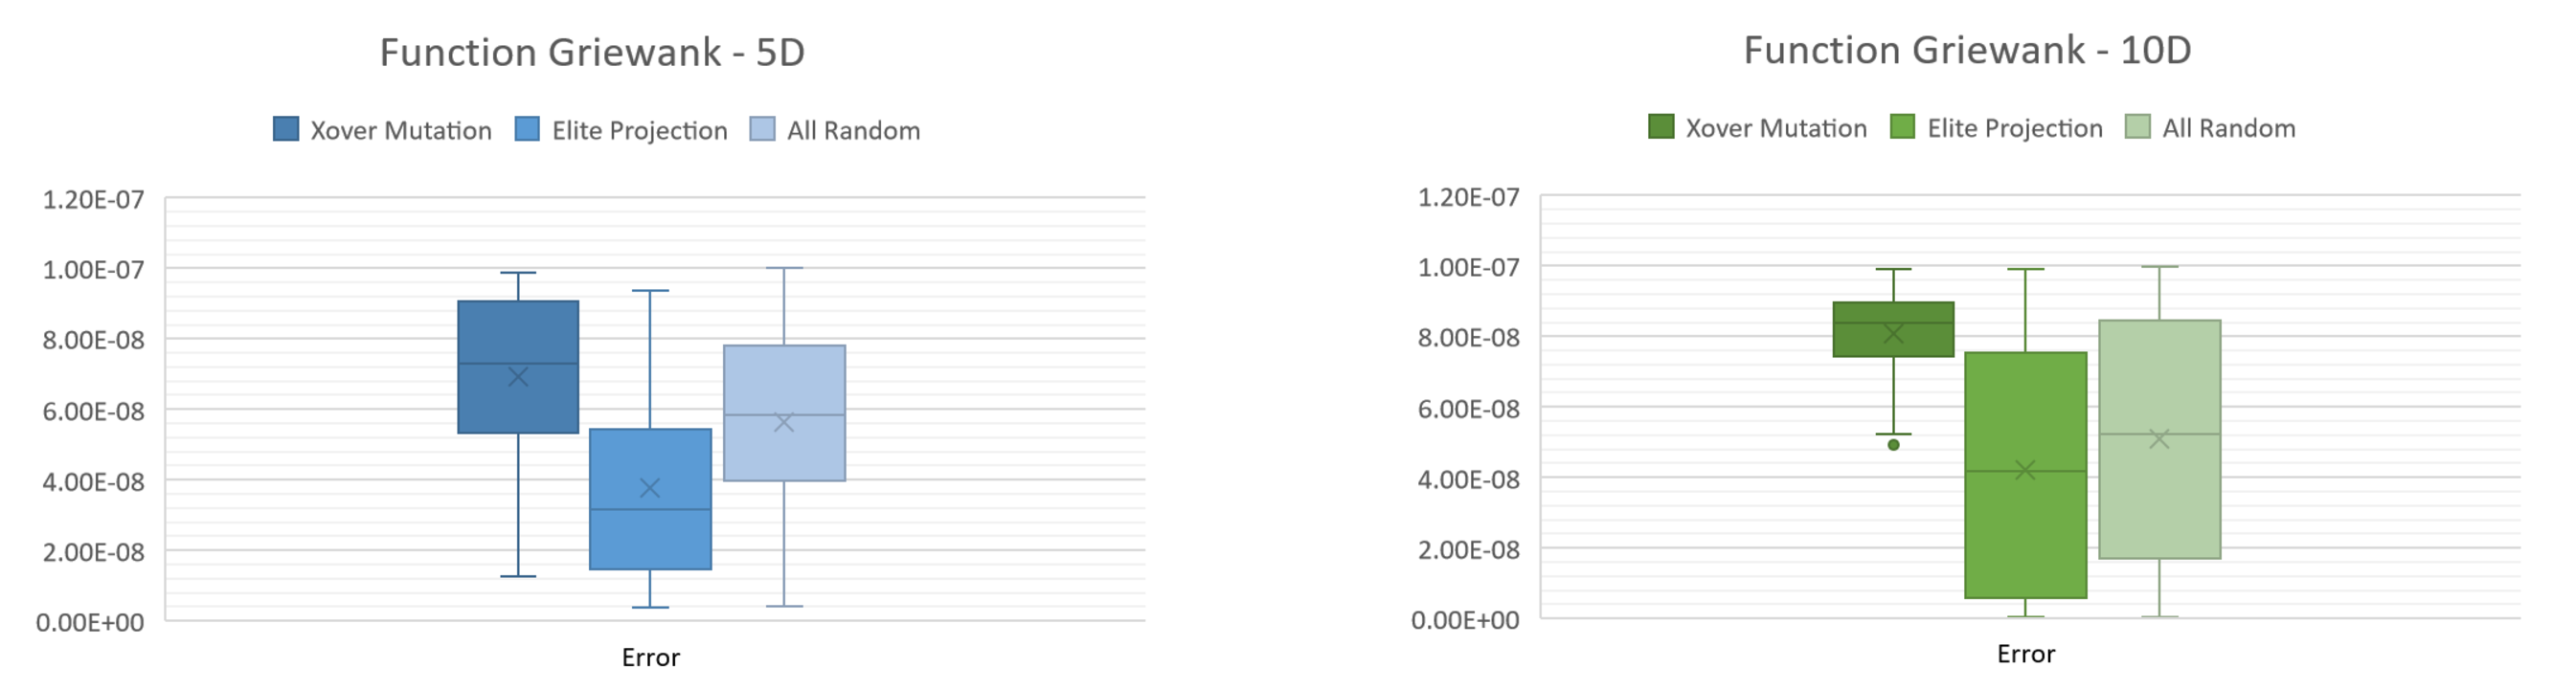
\includegraphics[width=0.99\linewidth, frame]{img/fig_fun_griewank.pdf}
                \caption{Box and whisker chart for the Griewank Benchmark Function, 5 vs 10 Dimensions.} \label{fig.fun_griewank}
                \end{figure}

            \begin{table}[]
                \scriptsize
                \centering
                \caption{Griewank Benchmark Function summarized experiments table for 5 Dimensions.}\label{tab.fun_griewank5}
                \begin{tabular}{@{}lllll@{}}
                \toprule
                \multicolumn{5}{l}{\textbf{Griewank Function - 5 Dimensions}} \\ \midrule
                & \textbf{Error} & \textbf{St-Dev} & \textbf{Evals.} & \textbf{Time} \\
                \textbf{Xover Mutation} & 6.92E-08 & 2.40E-08 & 44,566 & 48.3 \\
                \textbf{Elite Projection} & 3.77E-08 & 2.74E-08 & 16,412 & 20.1 \\
                \textbf{All Random} & 5.63E-08 & 2.99E-08 & 35,761 & 38.5 \\ \bottomrule
                \end{tabular}
                \end{table}

            \begin{table}[]
                \scriptsize
                \centering
                \caption{Griewank Benchmark Function summarized experiments table for 10 Dimensions.}\label{tab.fun_griewank10}
                \begin{tabular}{@{}lllll@{}}
                \toprule
                \multicolumn{5}{l}{\textbf{Griewank Function - 10 Dimensions}} \\ \midrule
                & \textbf{Error} & \textbf{St-Dev} & \textbf{Evals.} & \textbf{Time} \\
                \textbf{Xover Mutation} & 8.07E-08 & 1.39E-08 & 92,885 & 100.0 \\
                \textbf{Elite Projection} & 4.21E-08 & 3.40E-08 & 13,534 & 17.3 \\
                \textbf{All Random} & 5.08E-08 & 3.54E-08 & 40,544 & 52.5 \\ \bottomrule
                \end{tabular}
                \end{table}

            \FloatBarrier


        \subsubsection{Rastrigin Benchmark Function Experiment}

            This experiment's goal was to follow and study the behavior of our
            proposed strategy, to repeat the results in the same order as
            expected, in a reduced number of both time and evaluations. We
            selected Rastrigin Classic Benchmark Function for Optimization for
            this experiment. Figure~\ref{fig.fun_rastrigin} shows its
            corresponding Box and Whisker chart, where we summarized the
            results in Tables~\ref{tab.fun_rastrigin5} and~\ref{tab.fun_rastrigin10} 
            (for five and ten dimensions, respectively).

            \begin{figure}
                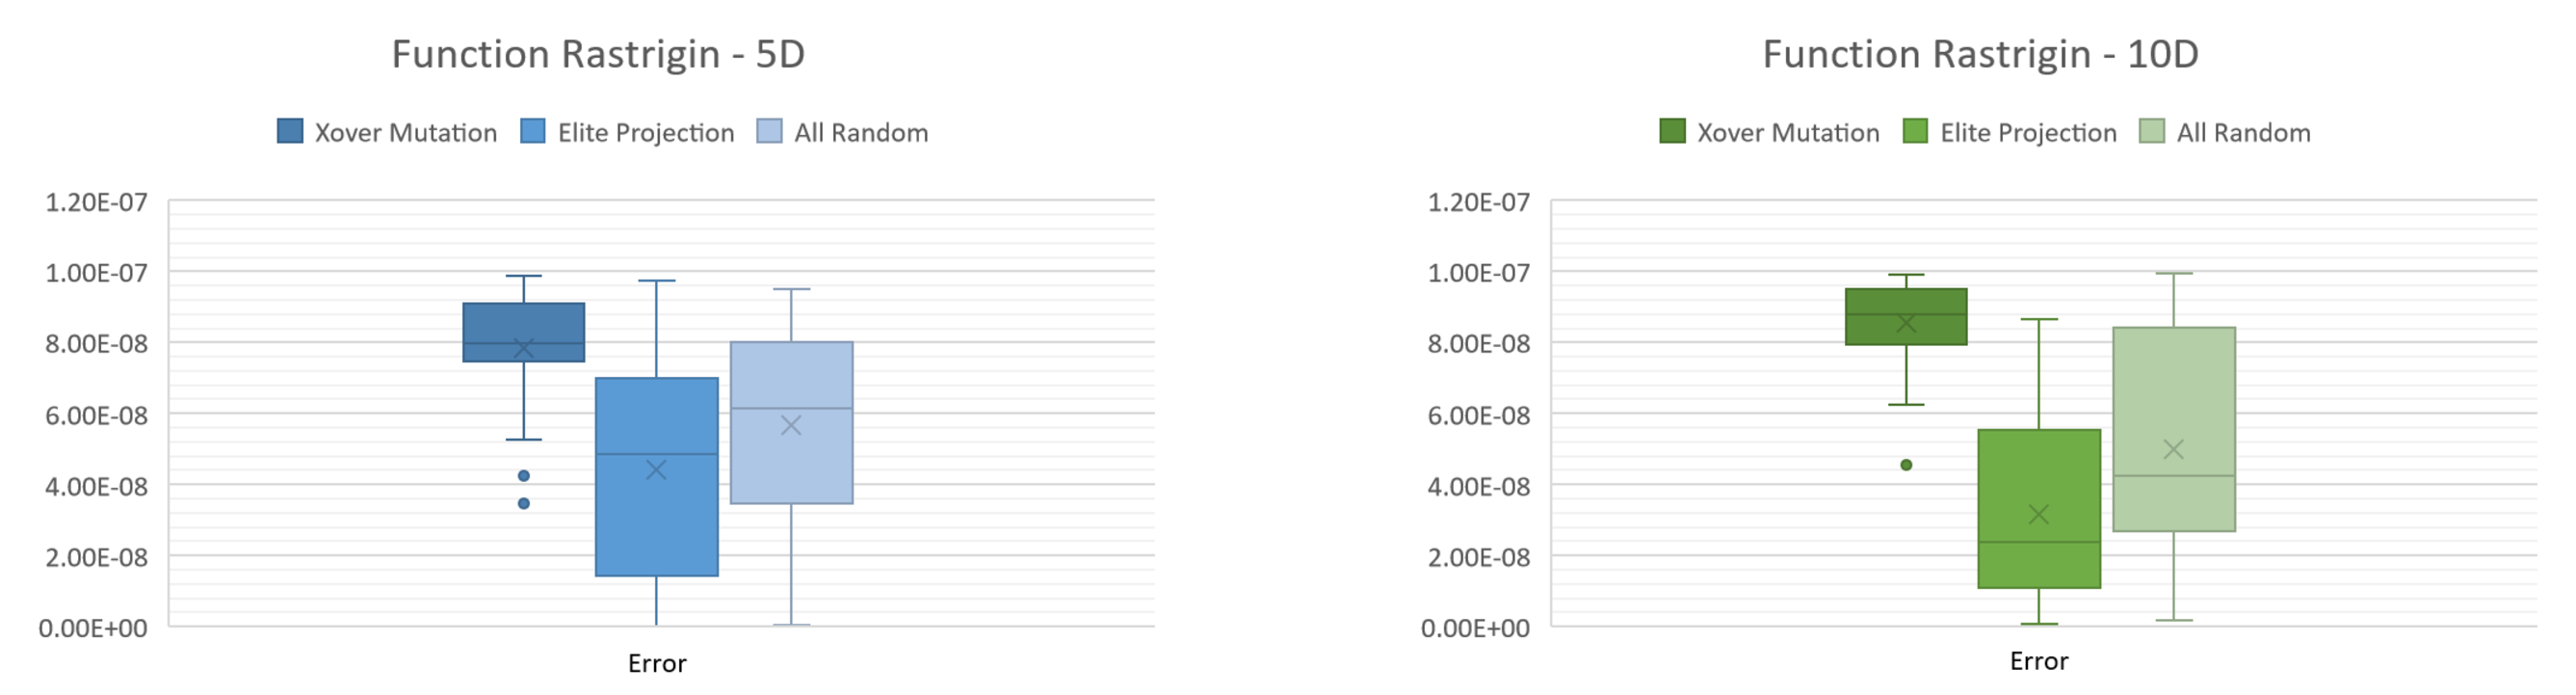
\includegraphics[width=0.99\linewidth, frame]{img/fig_fun_rastrigin.pdf}
                \caption{Box and whisker chart for the Rastrigin Benchmark Function, 5 vs 10 Dimensions.} \label{fig.fun_rastrigin}
                \end{figure}

            \begin{table}[]
                \scriptsize
                \centering
                \caption{Rastrigin Benchmark Function summarized experiments table for 5 Dimensions.}\label{tab.fun_rastrigin5}
                \begin{tabular}{@{}lllll@{}}
                \toprule
                \multicolumn{5}{l}{\textbf{Rastrigin Function - 5 Dimensions}} \\ \midrule
                & \textbf{Error} & \textbf{St-Dev} & \textbf{Evals.} & \textbf{Time} \\
                \textbf{Xover Mutation} & 7.85E-08 & 1.59E-08 & 22,322 & 34.1 \\
                \textbf{Elite Projection} & 4.42E-08 & 3.26E-08 & 10,860 & 14.8 \\
                \textbf{All Random} & 5.66E-08 & 2.81E-08 & 21,122 & 35.0 \\ \bottomrule
                \end{tabular}
                \end{table}

            \begin{table}[]
                \scriptsize
                \centering
                \caption{Rastrigin Benchmark Function summarized experiments table for 10 Dimensions.}\label{tab.fun_rastrigin10}
                \begin{tabular}{@{}lllll@{}}
                \toprule
                \multicolumn{5}{l}{\textbf{Rastrigin Function - 10   Dimensions}} \\ \midrule
                & \textbf{Error} & \textbf{St-Dev} & \textbf{Evals.} & \textbf{Time} \\
                \textbf{Xover Mutation} & 8.56E-08 & 1.23E-08 & 53,579 & 58.7 \\
                \textbf{Elite Projection} & 3.17E-08 & 2.57E-08 & 8,704 & 13.0 \\
                \textbf{All Random} & 5.00E-08 & 3.16E-08 & 24,376 & 27.4 \\ \bottomrule
                \end{tabular}
                \end{table}
            
            \FloatBarrier


        \subsubsection{Sphere Benchmark Function Experiment}

            For our fifth experiment we chose the Sphere Classic Benchmark
            Function for Optimization. Even though the sphere function is
            considered one of the simplest to solve, the same behavior was
            consistent for the algorithm, where it showed a reduced number of
            evaluations and execution time. We can confirm this affirmation
            with the results shown in this experiment.
            Figure~\ref{fig.fun_sphere} displays its corresponding Box and
            Whisker chart, where we summarized the results in
            Tables~\ref{tab.fun_sphere5} and~\ref{tab.fun_sphere10} (for
            five and ten dimensions, respectively).

            \begin{figure}
                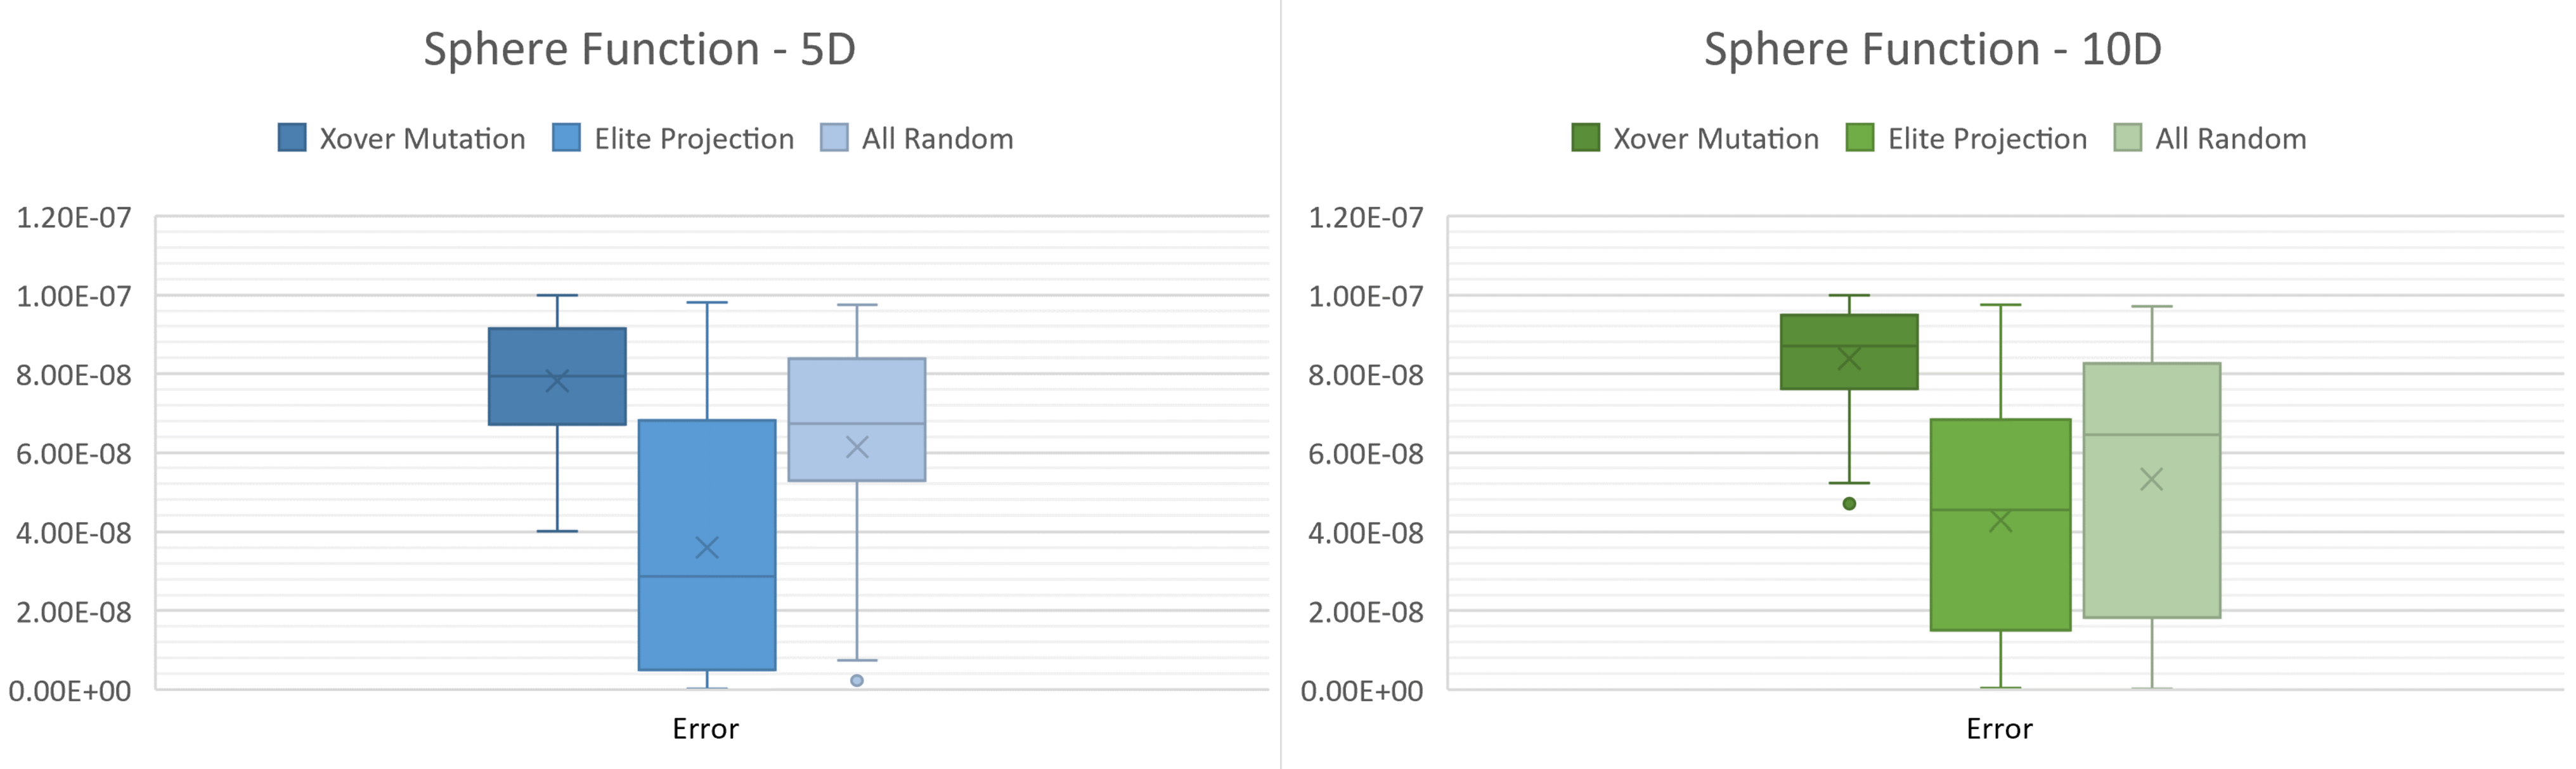
\includegraphics[width=0.99\linewidth, frame]{img/fig_fun_sphere.pdf}
                \caption{Box and whisker chart for the Sphere Benchmark Function, 5 vs 10 Dimensions.} \label{fig.fun_sphere}
                \end{figure}

            \begin{table}[]
                \scriptsize
                \centering
                \caption{Sphere Benchmark Function summarized experiments table for 5 Dimensions.}\label{tab.fun_sphere5}
                \begin{tabular}{@{}lllll@{}}
                \toprule
                \multicolumn{5}{l}{\textbf{Sphere Function - 5 Dimensions}} \\ \midrule
                & \textbf{Error} & \textbf{St-Dev} & \textbf{Evals.} & \textbf{Time} \\
                \textbf{Xover Mutation} & 7.82E-08 & 1.65E-08 & 11,312 & 14.5 \\
                \textbf{Elite Projection} & 3.60E-08 & 3.27E-08 & 7,056 & 10.9 \\
                \textbf{All Random} & 6.14E-08 & 2.79E-08 & 9,158 & 12.2 \\ \bottomrule
                \end{tabular}
                \end{table}

            \begin{table}[]
                \scriptsize
                \centering
                \caption{Sphere Benchmark Function summarized experiments table for 10 Dimensions.}\label{tab.fun_sphere10}
                \begin{tabular}{@{}lllll@{}}
                \toprule
                \multicolumn{5}{l}{\textbf{Sphere Function - 10 Dimensions}} \\ \midrule
                & \textbf{Error} & \textbf{St-Dev} & \textbf{Evals.} & \textbf{Time} \\
                \textbf{Xover Mutation} & 8.39E-08 & 1.45E-08 & 30,769 & 34.4 \\
                \textbf{Elite Projection} & 4.28E-08 & 3.06E-08 & 9,236 & 13.3 \\
                \textbf{All Random} & 5.32E-08 & 3.38E-08 & 21,465 & 26.3 \\ \bottomrule
                \end{tabular}
                \end{table}

            \FloatBarrier


        \subsubsection{Rosenbrock Benchmark Function Experiment}

            The goal of our sixth and last experiment was to study the behavior
            of the Animal Life-Cycle Algorithm when tested with the Rosenbrock
            Benchmark Function for Optimization. From all of our previous
            evaluation functions, Rosenbrock presented the most difficult
            challenge for our algorithm. This test facilitated the
            differentiation between the three compared strategies because the
            solutions found were in different numeric order. After all tests,
            the Elite Projection proved to be the best alternative. We can
            corroborate this by analyzing Figures~\ref{fig.fun_rosenbrock_5d}
            and~\ref{fig.fun_rosenbrock_10d}, which shows its corresponding Box
            and Whisker chart. We present the summarized results in
            Tables~\ref{tab.fun_rosenbrock5} and~\ref{tab.fun_rosenbrock10}
            (for five and ten dimensions, respectively).

            \begin{figure}
                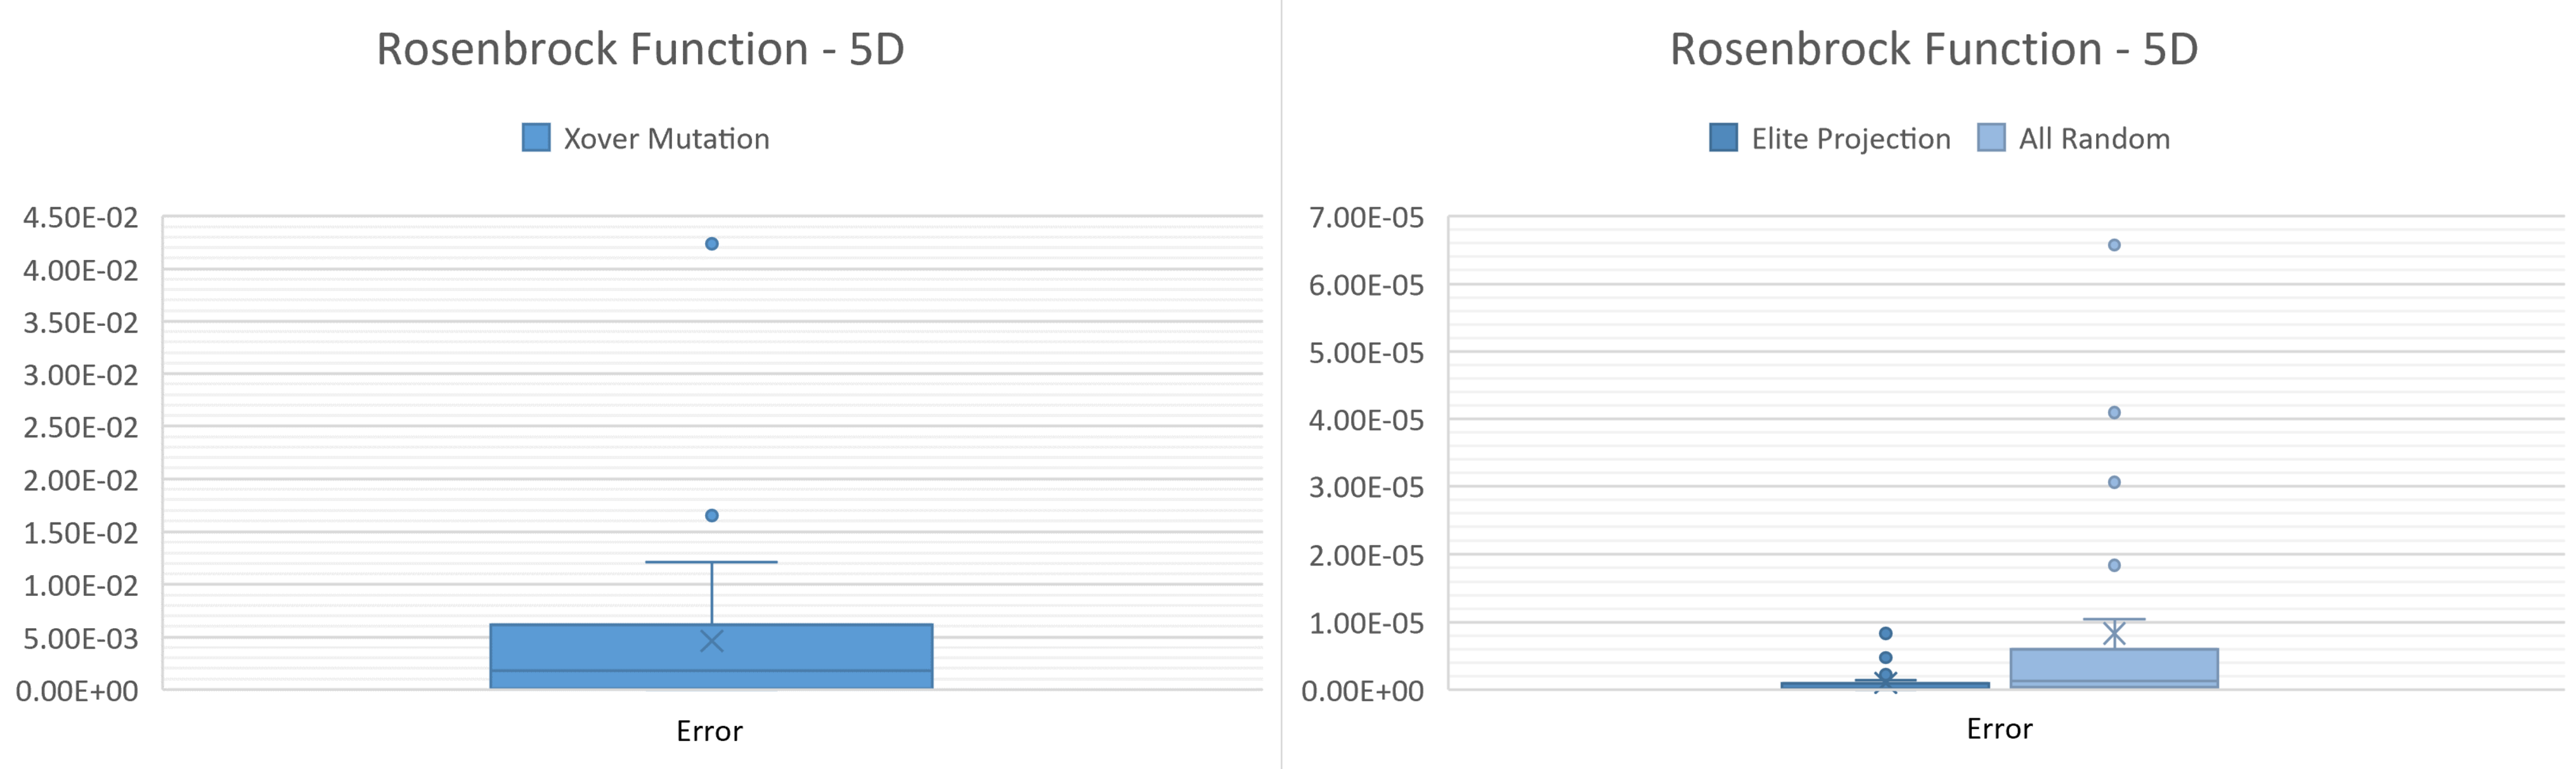
\includegraphics[width=0.99\linewidth, frame]{img/fig_fun_rosenbrock_5d.pdf}
                \caption{Box and whisker chart for the Rosenbrock Benchmark Function, 5 Dimensions.} \label{fig.fun_rosenbrock_5d}
                \end{figure}

            \begin{table}[]
                \scriptsize
                \centering
                \caption{Rosenbrock Benchmark Function summarized experiments table for 5 Dimensions.}\label{tab.fun_rosenbrock5}
                \begin{tabular}{@{}lllll@{}}
                \toprule
                \multicolumn{5}{l}{\textbf{Rosenbrock Function - 5 Dimensions}} \\ \midrule
                & \textbf{Error} & \textbf{St-Dev} & \textbf{Evals.} & \textbf{Time} \\
                \textbf{Xover Mutation} & 4.65E-03 & 8.29E-03 & 500,000 & 646.4 \\
                \textbf{Elite Projection} & 9.62E-07 & 1.86E-06 & 307,878 & 427.0 \\
                \textbf{All Random} & 8.30E-06 & 1.58E-05 & 491,400 & 697.8 \\ \bottomrule
                \end{tabular}
                \end{table}


            \begin{figure}
                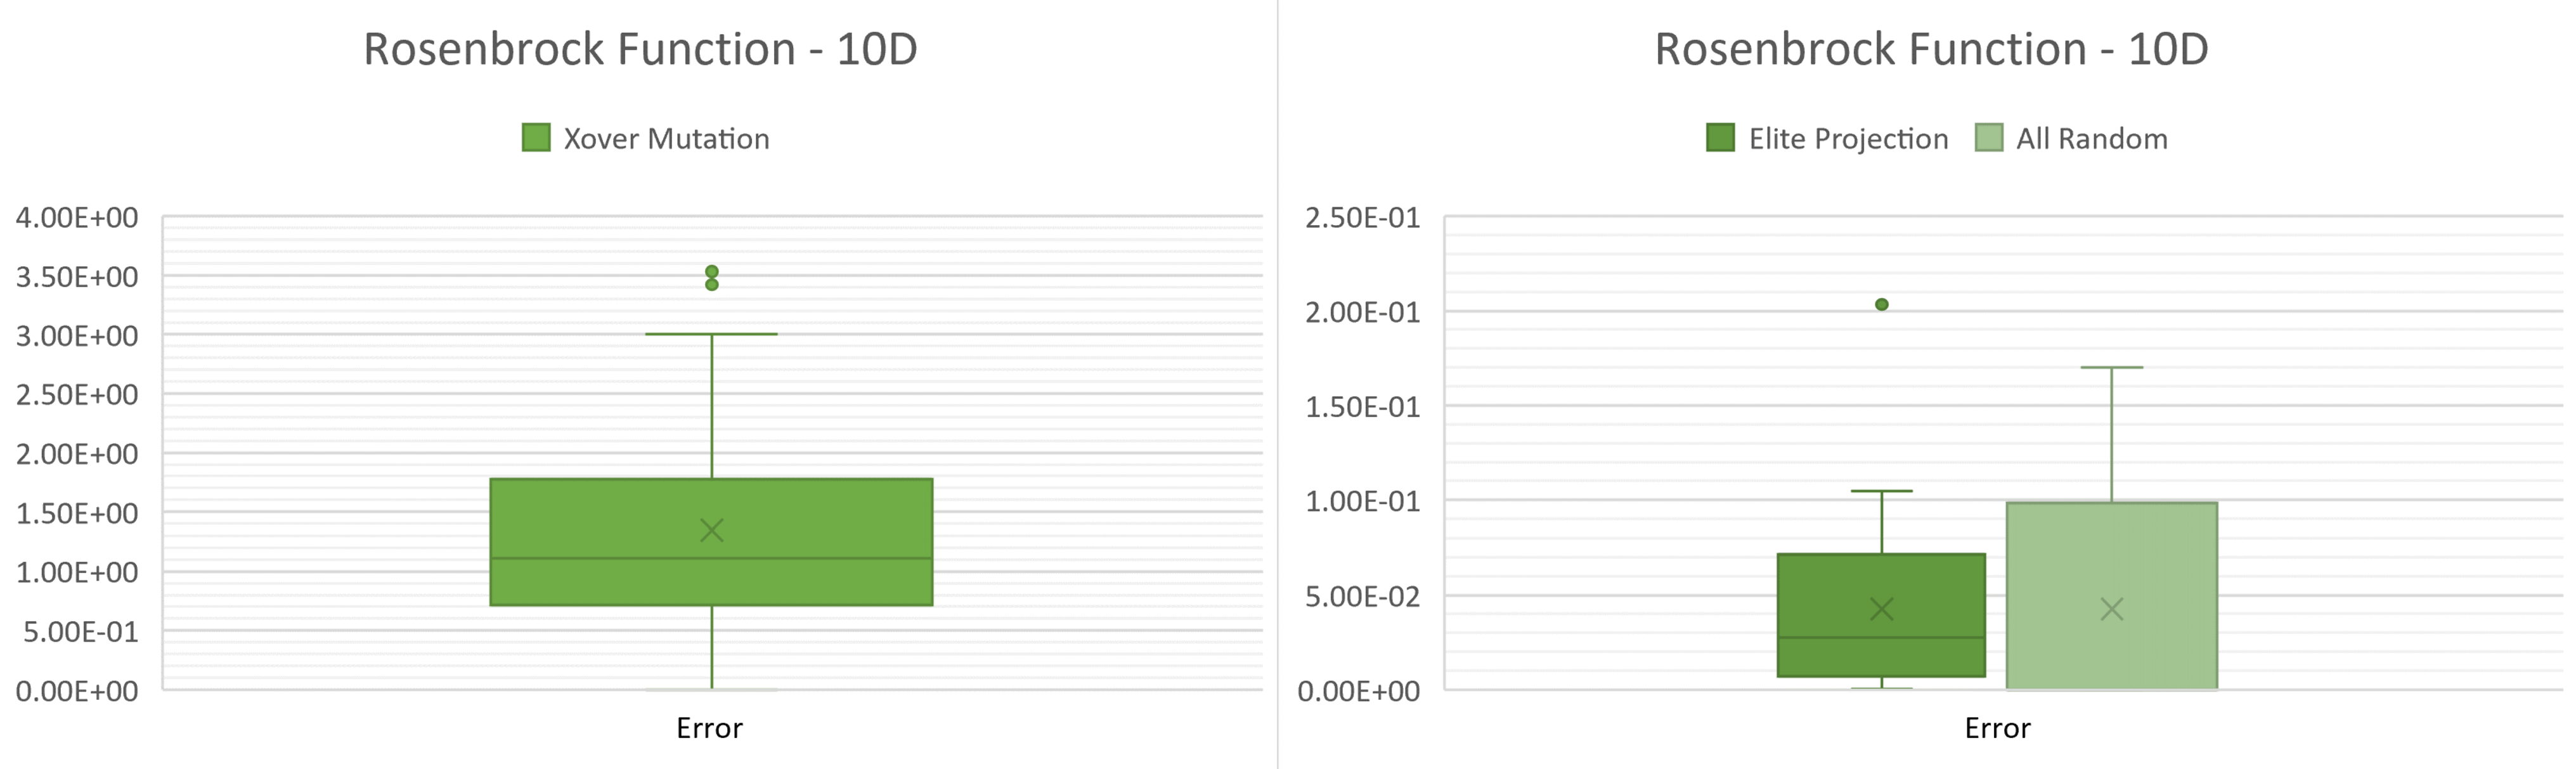
\includegraphics[width=0.99\linewidth, frame]{img/fig_fun_rosenbrock_10d.pdf}
                \caption{Box and whisker chart for the Rosenbrock Benchmark Function, 10 Dimensions.} \label{fig.fun_rosenbrock_10d}
                \end{figure}

            \begin{table}[]
                \scriptsize
                \centering
                \caption{Rosenbrock Benchmark Function summarized experiments table for 10 Dimensions.}\label{tab.fun_rosenbrock10}        
                \begin{tabular}{@{}lllll@{}}
                \toprule
                \multicolumn{5}{l}{\textbf{Rosenbrock Function - 10 Dimensions}} \\ \midrule
                & \textbf{Error} & \textbf{St-Dev} & \textbf{Evals.} & \textbf{Time} \\
                \textbf{Xover Mutation} & 1.35E+00 & 9.83E-01 & 1,000,000 & 1,384.3 \\
                \textbf{Elite Projection} & 4.26E-02 & 4.34E-02 & 1,000,000 & 1,146.0 \\
                \textbf{All Random} & 4.27E-02 & 6.02E-02 & 952,038 & 1,147.8 \\ \bottomrule
                \end{tabular}
                \end{table}
            
            \FloatBarrier

\section{Discussion}
    \label{section.discussion}

    Imagine being an astronaut on a mission repairing a space station in the
    middle of space. Suddenly, a block of asteroids hits the craft, and you
    lose your oxygen tank while the explosion pushes you away. From afar, you
    see the area where your tank might be, covered with something similar to a
    gas leaked from the station that blocks all visibility. Finding the tank is
    the only hope to return to your main ship some miles away. The oxygen
    reserve from your suit is running out, and there are only a couple of
    minutes left. Now hold your breath in real life and think, what strategy
    will you choose to search for your tank? We repeated this mental exercise
    several times until we found the best solution (or blacked out).

    If your life depended on it, would you choose a Genetic Algorithm, a
    variant of a Particle Swarm Optimization Algorithm, or another? We searched
    for a way to mix both, at least in some way, take the main idea or concepts
    from them and make them work together. We strongly believe it is possible
    to combine the features, as previous work has proven to obtain outstanding
    results \cite{garcia2015evospace,garcia2021event,valdez2021container,valdez2021swarm}.
    Our goal was to create a swarm out of the best individuals found in
    evolution. We probably have a long way to go, but at least we are getting
    promising results. From our experiments, all six Classic Benchmark
    Functions for Optimization (Ackley, Bohachevsky, Griewank, Rastrigin,
    Sphere, and Rosenbrock) proved the same behavior for the Animal Life Cycle
    Algorithm: finding the expected solution in a reduced number of evaluations
    and less execution time.


\section{Conclusions}
    \label{section.conclusions}

    The Animal Life Cycle Algorithm allows for multiple parameters'
    fine-tuning, facilitating the freedom to experiment with different
    alternatives to restart the population and solve extinction caused by
    nature's pressure, which will impact how quickly, and the quality of its
    found solution. We compared the results obtained with the use of historical
    elite projection versus other alternatives, using classic benchmark
    functions for optimization for comparison, where it showed favorable and
    promising results.

    As the nature of the challenge increases, it is indispensable to have an
    elastic, scalable, and fault-tolerant model designed with cloud
    collaboration processes, and asynchronous communication. We have proven
    that it is possible to evolve a population, using a distributed, parallel,
    and asynchronous strategy, inspired by the Genetic Algorithm (GA). To
    further validate this work, we could use some more demanding (or control)
    problem that requires calculating real numbers
    \cite{stanley2002evolving,miikkulainen2019evolving}. We implemented the
    algorithm using Docker containers.


\begin{acknowledgement}
    This paper has been supported in part by projects DeepBio (TIN2017--85727--C4--2--P) and TecNM Project 11356.21\@.
\end{acknowledgement}

% ---- Bibliography ----
% BibTeX users should specify bibliography style 'splncs04'.
% References will then be sorted and formatted in the correct style.
%

\bibliographystyle{splncs03_unsrt}
%\bibliographystyle{splncs04}
\bibliography{bib/bibliografia.bib}
%\bibliography{10.1007_978-3-031-08266-5_8-citation.bib}

\end{document}

% TO-DO: Turnitin.
